\documentclass[11pt, oneside]{article}   	% use "amsart" instead of "article" for AMSLaTeX format
\usepackage{geometry}                		% See geometry.pdf to learn the layout options. There are lots.
\geometry{letterpaper}                   		% ... or a4paper or a5paper or ... 
%\geometry{landscape}                		% Activate for for rotated page geometry
%\usepackage[parfill]{parskip}    		% Activate to begin paragraphs with an empty line rather than an indent
\usepackage{graphicx}				% Use pdf, png, jpg, or eps§ with pdflatex; use eps in DVI mode
								% TeX will automatically convert eps --> pdf in pdflatex		
\usepackage{amssymb}
\usepackage{amsmath}
\usepackage{parskip}
\usepackage{color}
\usepackage{hyperref}

\title{Karkhar Power Series Video}
%\author{The Author}
%\section{}
%\subsection*{}
\date{}							% Activate to display a given date or no date

\graphicspath{{/Users/telliott_admin/Dropbox/Tex/png/}}
% \begin{center} 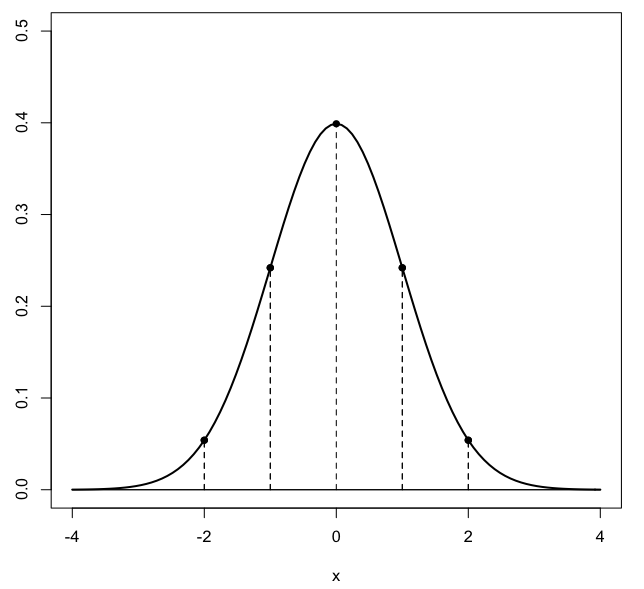
\includegraphics [scale=0.4] {gauss3.png} \end{center}
\begin{document}
\maketitle
\Large
Power series have a big role in complex analysis.  A standard power series is something like
\[ \sum_{n=0}^{\infty} a_n \ (z - z_0)^n \]
where $z_0$ is a fixed point in the Argand plane and $z$ is a variable.  This series will either converge for all $z$, converge only for $z = z_0$, or converge only for $| z - z_0 | < R$ (only for $z$ within some distance $R$ from $z_0$.  In the first case we say that the radius of convergence $R = \infty$.

Kharkar starts with the following theorem:

Suppose there is a $z_1 \ne z_0$ such that this series converges:
\[ \sum_{n=0}^{\infty} a_n \ (z_1 - z_0)^n \]
Then
\[ \forall \ z: |z - z_0| < |z_1 - z_0| \]
\[ \sum_{n=0}^{\infty} a_n \ (z - z_0)^n \ \text{converges absolutely} \]

To state this in words:  If we know a point $z_1$ away from $z_0$ where the series converges, then the series converges absolutely for \emph{every} point that is closer to $z_0$ than $z_1$ is.

\subsection*{Proof}
The distance in the plane between $z$ and $z_0$ is less than the distance between $z_1$ and $z_0$, so we find some real number $r$ which lies between these two values.  We know that this is possible no matter how close $z$ lies to $z_1$, because of the properties of the real numbers.

That is, for any point $z$ in the open disk centered on $z_0$ whose boundary contains $z_1$, we can find $r$ such that
\[ |z-z_0| \le r < |z_1-z_0| \]

Now, let's examine the infinite series at $z_1$ which is given to be convergent
\[ \sum_{n=0}^{\infty} a_n \ (z_1 - z_0)^n \]
A basic property of convergent series is that the individual terms must tend to zero.
\[ \lim_{n \rightarrow \infty} \ a_n \ (z_1 - z_0)^n = 0 \]
This in turn means that there must be a largest term of the series.  So we pick some upper limit, a number called $M$ which is equal to or larger than the largest term and then we can say that
\[ \ |a_n| \ |z_1 - z_0|^n \le M \ , \ \ \ \forall \ n \]
every term in the series is less than or equal to $M$.

Next we look at a general term in the series, take absolute values and multiply on the top and bottom by $|z_1 - z_0|^n$:
\[ |a_n| |z - z_0|^n = |a_n| |z_1 - z_0|^n \ \cdot \frac{|z - z_0|^n}{|z_1 - z_0|^n} \]
The first part of the right-hand side is less than or equal to $M$ for every term in the series:
\[ |a_n| |z - z_0|^n \le M \cdot \frac{|z - z_0|^n}{|z_1 - z_0|^n} \]

Now look at the second part of the right-hand side.  Recall that
\[ |z-z_0| \le r < |z_1-z_0| \]
Let
\[ p = \frac{r}{|z_1 - z_0|} < 1 \]
For every term, $|z - z_0| \le r$
so
\[ \frac{|z - z_0|}{|z_1 - z_0|} \le p < 1 \]
and then for every term
\[ |a_n| |z - z_0|^n \le M \cdot p^n \]
Looking now at the sum (remember that this is our interior point $z$):
\[ \sum_{n=0}^{\infty} |a_n| \ |(z - z_0)|^n < \sum_{n=0}^{\infty} M p^n <  M \sum_{n=0}^{\infty} p^n \]
The sum is seen to be a geometric series with ratio less than $1$, which we know converges.  Since term-by-term the left-hand side is less than the right-hand side, and the right-hand side converges, so does the left-hand side.
\[ \sum_{n=0}^{\infty} |a_n| \ |(z - z_0)|^n \]
converges, and then so does
\[ \sum_{n=0}^{\infty} a_n \ (z - z_0)^n \]
converge, absolutely.
$\square$
\subsection*{Convergence test}
The next section of the video takes a look at tests of convergence:  the ratio test and the root test.  The ratio test says to take the ratio of the absolute value of successive terms in the series.  If the ratio is less than one, the series converges.  (If greater than one, it diverges, and if equal to one, we can't say.)

Example:
\[ \sum_{n=0}^{\infty} (-1)^n \ \frac{z^n}{n!} \]
We need to find
\[ \lim_{n \rightarrow \infty} | \frac{(-1)^{n+1} z^{n+1} }{(n+1)!} \frac{n!}{(-1)^{n} z^{n}} | \]
The part of the quotient involving $(-1)^{n+1}/(-1)^n$ disappears because we take the absolute value.  That leaves
\[ \lim_{n \rightarrow \infty} | \frac{z^{n+1} }{(n+1)!} \frac{n!}{ z^{n}} | \]
\[ = \lim_{n \rightarrow \infty} | \frac{z}{n+1} | \]
For any $z$, this limit is zero, so we say that the series converges and it has a radius of convergence $R = 0$.

For the root test, consider this example:
\[ \sum_{n=0}^{\infty} 5^n (z-1)^n \]
The test says to consider the limit of the nth root of the absolute value of the nth term
\[ \lim_{n \rightarrow \infty} |5^n (z-1)^n |^{1/n} = 5 |z-1| \]
Again, we obtain convergence when this limit is less than one so
\[ 5 |z-1| < 1 \]
\[ |z - 1| < \frac{1}{5} \]
The radius of convergence is a circle of radius $1/5$ around the point $1$.

\subsection*{Derivative of a power series}
Kharkar first says that if the radius of convergence is $R$, then inside the disk $|z - z_0 < R|$ the function
\[ f(z) = \sum_{n = 0}{\infty} a_n (z - z_0)^n \]
is \emph{infinitely differentiable}.

If $f(z)$ has a positive (or infinite) radius of convergence, then inside the disk $|z-z_0| < R$, $f(z)$ is infinitely differentiable, and each derivative is given by a power series:
\[ f^{(k)}(z) = \sum_{n=k}^{\infty} n(n-1) \dots (n-k+1) \ a_n \ (z-z_0)^{n-k} \]
Consider as an example this power series with $a_n = n$:
\[ f(z) = \sum_0^{\infty} n \ z^n = 0 + z + 2z^2 + 3z^3 \dots \]
Differentiate term by term:
\[ f'(z) = 1 + 2^2 z + 3^2 z^2 + \dots + n^2 z^{n-1} + \dots \]
Does this match the definition?
\[ f^{(k)}(z) = \sum_{n=k}^{\infty} n(n-1) \dots (n-k+1) \ a_n \ (z-z_0)^{n-k} \]
The first derivative is for $k=1$ so
\[ n \dots (n-k+1) = n \]
and $z_0 = 0$ so
\[ f'(z) = \sum_{n=1}^{\infty}n \ a_n \ z^{n-1} \]
Recall that $a_n = n$
\[ = \sum_{n=1}^{\infty}n^2 \ z^{n-1} \]
which indeed matches
\[ f'(z) = 1 + 2^2 z + 3^2 z^2 + \dots + n^2 z^{n-1} + \dots \]

Go back to 
\[ f^{(k)}(z) = \sum_{n=k}^{\infty} n(n-1) \dots (n-k+1) \ a_n \ (z-z_0)^{n-k} \]
If $z = z_0$ then
\[ f^{(k)}(z_0) = \sum_{n=k}^{\infty} n(n-1) \dots (n-k+1) \ a_n \ 0^{n-k} \]
Now you might think that all these terms would be zero, and they are provided that $n-k \ne 0$, but there:
\[ f^{(k)}(z_0) = \sum_{n=k}^{\infty} n(n-1) \dots 1 \ a_n \ 0^{0} \]
\[ f^{(k)}(z_0) = n! \ a_n\]
\[ a_n = \frac{1}{n!} \ f^{(k)}(z_0)  \]
And the reason is that 
\[ 0^0 = \lim_{n \rightarrow 0} n^n = 1 \]
\url{http://mathforum.org/dr.math/faq/faq.0.to.0.power.html}

\subsection*{exponential}
Write the exponential as
\[ e^z = \sum_{n=0}^{\infty} \frac{z^n}{n!} = 1 + z + \frac{z^2}{2} + \frac{z^3}{3} + \dots \]
We could use the formula for the derivative, or just differentiate term by term and obtain that
\[ f(z) = f'(z) \]
Now write
\[ \ [ \ e^{-z} f(z) ] ' = -e^{-z} f(z) + e^{-z} f'(z) \]
(by the chain rule) and since 
\[ f(z) = f'(z) \]
we see that the right-hand side 
\[ -e^{-z} f'(z) + e^{-z} f'(z) = 0 \]
is just 0.  So that means the original compound function is a constant, since its derivative is zero:
\[ e^{-z} f(z) = C \]
and this is true for any $z$ so for $z=0$ we have
\[ e^0 f(0) = f(0) = C \]
so going back to the series, when $z=0$
\[ f(0) = \sum_{n=0}^{\infty} \frac{z^n}{n!} = \sum_{n=0}^{\infty} \frac{0^n}{n!} \]
Now, the numerator is zero for all terms except $n=0$ where it is equal to $1$ (see above), and that denominator is $0! = 1$, so 
\[ f(0) = 1 = C \]
Thus
\[ e^{-z} f(z) = 1 \]
\[ f(z) = e^z \]



\end{document}